\documentclass[../main.tex]{subfiles}
\begin{document}
\newpage
\thispagestyle{empty}
\begin{center}
    {
\includegraphics[width=0.5\textwidth]{Imagenes/Logo UMA.jpg}\par}
    \vspace{1cm}
    {\bfseries\LARGE \Facultad \par}
    \vspace{0.5cm}
    {\scshape\Large \Grado \par}
    \vspace{1.5cm}
    {\scshape\Huge Anexo II \par}
    \vspace{0.5cm}
    {\scshape\Huge Diseño de Instalación de Saneamiento \par}
    \vspace{1.5cm}
    {\itshape\Large \TituloProyecto \par}
    \vfill
    {\Large Solicitante: \par}
    {\Large \Solicitante  \par}
    \vspace{1cm}
    {\Large Autores: \par}
    {\Large \Autora \par}
    {\Large \Autor \par}
    \vfill
    {\Large \Fecha \par}
\end{center}
\newpage

\section{Introducción}

En este anexo se ha realizado los cálculos necesarios para el diseño y la realización del saneamiento de aguas residuales así como pluviales en la instalación de una carpintería de madera.

Para realizar dicho anexo, se ha empleado el 'Documento básico de Salubridad' en su actualización del 14 de junio de 2022 por el Ministerio de Transportes, Movilidad y Agenda Urbana.

\section{Saneamiento Pluvial}

El primer paso a la hora de realizar un saneamiento pluvial es conocer las zonas que van a necesitar una evacuación de dichas aguas pluviales. Para este estudio, ambas cubiertas de la nave y el aparcamiento frente a la carpintería. 

Las zonas que se han designado son:

\begin{table}[H]
    \centering
    \begin{tabular}{c|c}
         Zona & Superficie en proyección horizontal [$m^2$] \\ \hline
         Cubierta 1 & 420 \\
         Cubierta 2 &  420 \\
         Aparcamiento & 546 \\
    \end{tabular}
    \caption{Superficies}
\end{table}

\subsection{Mapa de isoyetas y zonas pluviometricas}

El mapa de isoyetas es la representación de la distribución de las precipitaciones. Es necesario a la hora de dimensionar el saneamiento pluvial. 

\begin{figure}[H]
    \centering
    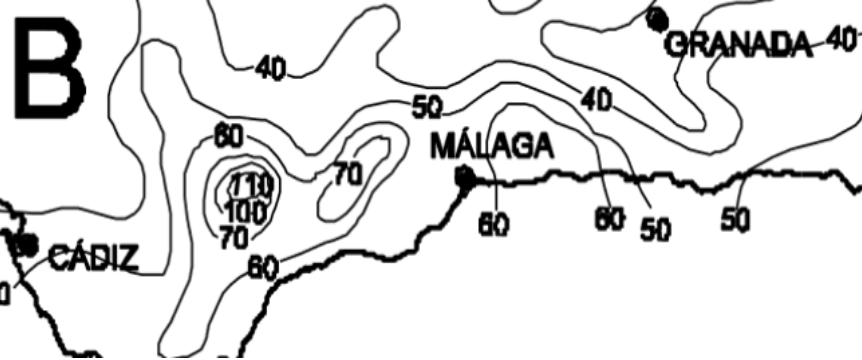
\includegraphics[width=1\linewidth]{Imagenes/detalleisoyetas.png}
    \caption{Detalle del mapa de Isoyetas}
\end{figure}

Cómo se puede apreciar tanto la ciudad de Málaga, como su polígono, se encuentran en la zona B y con una isoyeta de 50. Por tanto le corresponde una intensidad pluviométrica de 110 mm/h.

\subsubsection{Factor de corrección}

Se obtiene un factor de corrección debido a que la intensidad pluviométrica obtenida no es igual a 100 mm/h

\begin{equation}
    f = \frac{i}{100} = \frac{110}{100} = 1.1
\end{equation}

Donde

\begin{itemize}
    \item i = Intensidad pluviométrica en mm/h
    \item f = Factor de corrección aplicable a las superficies
\end{itemize}

\subsection{Canalón}

El diámetro del canalón depende de la cantidad de superficie en plano que debe de cubrir así como de la pendiente que este tenga. Para obtener el diámetro necesario se sigue la siguiente tabla para una pendiente de un 1\%.

\begin{table}[H]
    \centering
    \begin{tabular}{c|c|c}
         Msph [$m^2$] para 100 mm/h & Msph [$m^2$] para 110 mm/h & Diámetro nominal del canalón[mm] \\ \hline
         45 & 40.90 & 100 \\
         80 & 72.72 & 125 \\
         125 & 113.63 & 150 \\
         260 & 236.36 & 200 \\
         475 & 431.81 & 250 \\
    \end{tabular}
    \caption{Tabla para el diámetro del canalón}
\end{table}

Donde: 
\begin{itemize}
    \item Msph: Máxima superficie en proyección horizontal 
\end{itemize}

En el cuadro 2, la columna de la izquierda indica la máxima cantidad de superficie en proyección horizontal que un canalón con una pendiente del 1\% es capaz de cubrir para unas intensidad pluviométrica de 100 mm/h.

La columna central indica lo mismo pero tras ser realizado el factor correctivo obtenido anteriormente.

Por último, la columna de la derecha indica el diámetro nominal del canalón a colocar en $mm^2$

Por tanto, el canalón necesario para despejar el agua en ambos lados de la cubierta debe de ser de un diámetro nominal de 250 $mm^2$ o superior. 

Se decide de instalar un canalón de 25 cm de diámetro de PVC. 

\subsection{Bajante}

\begin{table}[H]
    \centering
    \begin{tabular}{c|c|c}
    Sph [$m^2$] para 100 mm/h & Sph [$m^2$] para 110 mm/h & Diámetro nominal de la bajante [mm] \\ \hline
    65&59.1&50 \\
    113&102.72&63 \\
    177&160.9&75 \\
    318&289.1&90 \\
    580&527.27&110 \\
    \end{tabular}
    \caption{Diámetros correspondiente a la superficie}
\end{table}

Donde:

\begin{itemize}
    \item Sph: Superficie en proyección horizontal
\end{itemize}

Si bien es cierto, que una única bajante podría ser capaz de desalojar toda el agua de la cubierta, esta opción no es recomendable. Ya que podría quedar total o parcialmente obstruida. Es por ello, que se ha decidido instalar un total de 6 bajantes. 3 a cada lado de las cubiertas.

Cada bajante cubre una superficie en proyección horizontal de 140 $m^2$, esto para una intensidad pluviometrica de 110 mm/h, corresponde con un diámetro nominal de la bajante de 75 mm.

Las bajantes acaban en un bote a pie de estas, no sifónico.

\subsection{Colectores}

\subsubsection{Cubiertas}

Los colectores se han calculado desde los bajantes más lejanos a la entrada a los más próximos, teniendo en cuenta la suma de la superficie total en proyección horizontal.

Los colectores son enterrados, por tanto, la pendiente mínima es de 2\%.

En la siguiente tabla, ya adaptada para 110 mm/h, se muestra, en función del porcentaje de pendiente que tenga el colector y la superficie en proyección horizontal, cuál tiene que ser el diámetro del colector.

\begin{table}[H]
    \centering
    \begin{tabular}{c|c|c}
    Msph [$m^2$] para un 2\% & Msph [$m^2$] para un 3\%  & Diámetro nominal del colector[mm] \\ \hline
    161.11 & 230 & 90 \\
    293.63 & 416.36 & 110 \\
    400 & 563.63 & 125 \\
    783.63 & 1136.36 & 160 \\
    1372.72 & 1945.45 & 200 \\
    
    \end{tabular}
    \caption{Diámetro del colector en función de la superficie y la pendiente}
\end{table}

Donde:

\begin{itemize}
   \item  Msph: Máxima superficie en proyección horizontal 
\end{itemize}

Cómo cada bajante cubre una superficie en proyección horizontal de 140 $m^2$, después del bote, no sifónico, colocado a pie de estas. Por tanto, el colector de cada una es de un diámetro de 90 mm, con una pendiente de un 2\%. 

Ambos colectores acaban en un bote, el colector saliente, debe de transportar la intensidad caída en la suma de ambas superficies, en este caso, una superficie en proyección horizontal total de 280 $m^2$. Para ello es necesario un colector de diámetro 110 mm, con una pendiente del 2\%.

Este colector llega a otro bote, que es abastecido por, otras dos colectores provenientes de una bajante, cada una cubre una superficie de 140 $m^2$ en proyección horizontal. Sumando un total de 560 $m^2$, el colector necesario es uno de diámetro nominal 125 mm y con un 3\% de pendiente.

Este colector, llega a un tercer bote, donde también llegan otros dos colectores provenientes de una bajante. La suma total de superficie es la de toda la cubierta en proyección horizontal, sumando un total de 840 $m^2$. El colector necesario es uno de 160 mm y de un 3\% de pendiente.

Con esto queda terminado la parte de ambas cubiertas.

\subsubsection{Aparcamientos}

Para los aparcamientos, se ha dividido en 4 subzonas.

\begin{table}[H]
    \centering
    \begin{tabular}{c|c}
         Nombre & Superficie [$m^2$] \\ \hline
         Zona 1 & 142.5 \\
         Zona 2 & 123.5\\
         Zona 3 & 130\\
         Zona 4 & 150\\
    \end{tabular}
    \caption{Subzonas del aparcamiento}
\end{table}

Se procede a instalar a cada zona un sumidero, el colector de cada uno de estos es de 90 mm con una pendiente del 2\%.

El colector de la zona 3 y de la zona 4, son conectados a un bote, de dicho bote sale un colector de 110 mm de diámetro y una pendiente del 2\%.

El colector de la zona 1, el de la zona 2 y el colector saliente del anterior bote, se unen en otro bote, del que sale un tercer colector de 125 mm de diámetro y 3\% de pendiente.

\subsection{Pozo general y acometida}

Se tienen 2 colectores:

\begin{itemize}
    \item Colector 1: Cubiertas. Con un diámetro de 160 mm.
    \item Colector 2: Aparcamiento. Con un diámetro de 125 mm.
\end{itemize}

Ambos son conectados al pozo general del edificio. De este sale una acometida, destinada ya la red pública. El colector entre ambos es de 200 mm de diámetro y con una pendiente del 2\%

\section{Saneamiento Residuales}

El primer paso para realizar el saneamiento residual es separar por zonas, las distintas instalaciones de fontanería realizadas.

\begin{table}[H]
    \centering
    \begin{tabular}{c|c|c|c}
    Zona & nº de Inodoros & nº de Lavabos & nº de Duchas \\ \hline
    Baño público masculino & 4 & 2 & 0 \\
    Baño público femenino & 4 & 2 & 0 \\
    Baño público discapacitados & 1 & 1 & 0 \\
    Vestuario hombres & 0 & 2 & 4 \\
    Vestuario mujeres & 0 & 2 & 4 \\
    \end{tabular}
    \caption{Zonas y sus instalaciones de fontanería}
\end{table}


\subsection{Derivaciones individuales}

\subsubsection{Baño masculino y femenino}

Siendo ambos idénticos, lo que se realice en uno, para el otro es igual. 

El primer paso es conocer cuantas UD o Unidades de Desagüe son necesarias desalojar, para ello hay que conocer:

\begin{itemize}
    \item Inodoro público con cisterna: 5 UD, con un sifón y derivación individual de 100 mm 
    \item Lavabo público: 2 UD, con un sifón y derivación individual de 40 mm
\end{itemize}

Multiplicando el número de UD por el número de instalaciones, se tiene un total de: 24 UD. 

\subsubsection{Baño de minusválidos}

El primer paso es conocer cuantas UD o Unidades de Desagüe son necesarias desalojar, para ello hay que conocer:

\begin{itemize}
    \item Inodoro público con cisterna: 5 UD, con un sifón y derivación individual de 100 mm 
    \item Lavabo público: 2 UD, con un sifón y derivación individual de 40 mm
\end{itemize}

Obtenido un total de 7 UD.

\subsubsection{Vestuarios}

Siendo ambos idénticos, lo que se realice en uno, para el otro es igual. 

El primer paso es conocer cuantas UD o Unidades de Desagüe son necesarias desalojar, para ello hay que conocer:

\begin{itemize}
    \item Ducha pública: 3 UD, con un sifón y derivación individual de 50 mm 
    \item Lavabo público: 2 UD, con un sifón y derivación individual de 40 mm
\end{itemize}

Obtenido un total de 16 UD. Esto sería para cada vestuario.

\subsection{Bajantes vestuarios}

Debido a que los vestuarios se encuentran en una entreplanta, es necesario una bajante. Para ello, se emplea una bajante de 63 mm de diametro, la cual su número máximo de UD es de 19 UD.

\subsection{Colectores horizontales}

Para ambos baños se escoge un colector horizontal de diámetro 63 mm, que posee capacidad de hasta 29 UD con una pendiente del 4\%

Para el baño de minusváliddos se escoge un colector horizontal de diámetro 50 mm, que posee una capacidad de hasta 20 UD con una pendiente del 2\%

Estos tres colectores se unen, en un colector que debe portar un total de 55 UD. Para ello, se desgina un colector de diámetro 90 mm, con una pendiente del 2\% y con capacidad para llevar hasta 96 UD.

A este último colector, previo al pozo general, se le añade los provenientes del vestuario, 16 UD cada una. Un total de 87 UD, por tanto, pueden añadirse al propio colector de diámetro 90 mm y pendiente del 2\%. 

Del pozo general, iría a la acometida con un diámetro identico de 90 mm y pendiente del 2\%


\end{document}